% !TEX root = _main.tex

\section{はじめに}

近年，音楽や映画といった時系列メディアを対象とした多様な作品分析手法が提案されている．これらの分析において，対象作品の視聴や分析方法の検討など，さまざまな要素が含まれるが，場面分けは多くの分析手法に共通する作業である．分析の手法として自動で行う手法と手動で行う手法が存在する．自動分割の課題として場面分けが細かすぎたり，複数の解釈の視点が存在したりする．そこで，場面分けをする際人の介入が必要となる．

そこで本研究では，人の解釈の介入が存在する手動で場面分けされていたものはどういった手法が存在するのか文献調査を行う．そして，そこから抽出された場面分けの切り方を参考に，1つの作品を対象として比較分析を行い，考察を行っていく．


\section{研究背景}
時系列メディアを扱った分析はさまざまな手法で行われている．分析をする上で様々な作業があるが，対象作品の場面分けは多くの分析手法に共通するものである．場面分けの手法として，自動で分割する方法と手動で分割する方法が存在する．

自動分割の例として，PySceneDetect\cite{PySceneDetect}が挙げられる．このツールは，動画からシーンの変更点を検出して，それに基づいて動画をシーン単位で分割することができるPythonライブラリである．動画編集や分析，コンテンツ管理などに応用されている．

シーン間の変化の閾値を設定することで，視覚的に大きな変化を特定可能となり，場面分けを行う．

PySceneDetectなどといった場面を自動で分割するシステムの課題として，場面分けが1秒や2秒になってしまい，一つ一つの場面が細かくなってしまうことが問題となる．また，分析を行う際，複数の解釈が存在するため場面のグルーピングの方針を検討する必要がある．

そこで，場面分けをする際人の解釈の介入が必要となる．つまり，自動分割した場面分けにさらに手動で分割やグルーピングをする必要がある．

\section{文献調査}\label{sec:related_works}
人の解釈の介入が存在する手動で分析された場面分けものはどのような手法で行われているのか調べるために文献調査を行った．

調査方法として，CiNii\cite{CiNii}iを利用し，手動によるメディア分析を対象とした論文を抽出・調査した．分析対象は以下の8つのカテゴリに絞った：演劇，小説，プレゼンテーション，映画，将棋，映像，作品分析，感情分析．これらの論文から，さらに「分析」と「場面分け」に関する記載があるものを抽出し，対象を絞り込んだ．

次に，抽出された論文に記載された場面分けに着目し，各分析者がどのような観点や理論に基づいて作品の場面分けを行っているのかを調査を行った．その結果，該当する論文は合計84件が抽出された．そのうち，「分析」と「場面分け」に関する記載が明確に認められる論文は12件に絞られた．これら12件の対象となるメディアのカテゴリは，映画，アニメ，ゲームシナリオ，ミステリー小説，ミュージカル，神話の6つであった．

以下で取り扱ったメディア分析を行っている論文のいくつかを例に挙げて概要，分析方法，場面分けのやり方を述べていく．

\subsection{論文例}
\subsubsection{長編アニメーション映画『崖の上のポニョ』の構造分析―2編の小さな異郷訪問譚の接合―}
\paragraph*{(1)概要}
スタジオジブリ製作における宮崎駿が関わった長編アニメーション映画には根強い人気がある．その中でも『崖の上のポニョ』を対象として構造分析を行う\cite{ponyo}．物語形式の中でも，「異郷訪問譚」の裏返し構造を用いた分析を行うことで，作品の特性を明らかにする．異郷訪問譚とは日本の代表的な異郷訪問譚である「イザナギの黄泉国訪問譚」や「浦島子」などにもみとめ られるように，古くから使用されてきた物語類型 の一つとも言え，いわゆる成長物語との関連がし ばしば指摘されてきた形式である．
\paragraph*{(2)分析方法}
物語の前半のテーマが後半では逆の順序で出現し，後半では前半の否定ないし対立という形をとる構造を裏返し構造という．その構造を援用する手法により『崖の上のポニョ』を分析していく．
\paragraph*{(3)場面分けの方法}
物語を前半と後半で分けその反対の形をとる場面の名称付けをして当てはめていく．

\subsubsection{物語の訴求分析の理論と手法及び応用事例}
\paragraph*{(1)概要}
物語は，古くから社会や文化の価値観形成に影響を与えてきた重要な要素．神話や昔話だけでなく，現代の娯楽作品（小説，コミック，アニメ，映画など）や広告，ニュース記事にも「物語」が含まれている．これらの物語は時代や文化に応じて変化し，私たちの価値観や意思決定に影響を与える\cite{sokyu}．「物語の訴求力」つまり，物語が持つ魅力や影響力を分析するための理論と手法を構築し，その意義を探ることを目的としている．
\paragraph*{(2)分析方法}
コミックの「進撃の巨人」を対象としてシーケンス分析を行っていく．シーケンス分析とは，物語が持つ「イベントの連鎖」に注目し，その構造を明らかにする分析手法である．この手法は，特に神話や民話などに見られる繰り返しのパターン（スキーマ）を抽出し，それがどのように物語全体の訴求力を形成しているかを検討することを目的とする．シーケンス分析は，物語の中に隠されたテーマや価値観を発見し，それを科学的に解明するための有力な手段となる．
\paragraph*{(3)場面分けの方法}
信頼や疑念といったスキーマを設定し，その内容に当てはまる場面を簡潔な言葉で設定した．

\subsection{結果}


以下で文献調査によって選定された論文の場面の切り方とグルーピング方法についてまとめていく．

\paragraph*{(1)長編アニメーション映画『崖の上のポニョ』の構造分析\cite{ponyo}}

切り方：『崖の上のポニョ』のあらすじを文章単位で区切る

グルーピング：登場人物をマーキングし，裏返しの関係を探る

\paragraph*{(2)神話物語と神話を原型にした現代物語の構造比較\cite{sinwa}}

切り方：物語内の事象（場所/部隊の移動・物語内時間が不連続となる時間経過）

グルーピング：課題の構成要素（発生・目的など）を抽出

\paragraph*{(3)ネットワーク分析を用いたミステリー小説における場面の依存関係の分析\cite{misuteri}}

切り方：物語内の事象（物語内での時間経過・特殊な事象/現象の発生・場面内で行動する人物の増減・主体や主観の変更・物語内での場所の移動）

グルーピング：依存場面を抽出

\paragraph*{(4)ロールプレイングシナリオにおけるクエスト構造に着目した物語分析\cite{rpg}}

切り方：ゲームシナリオ内のクエストで区切る

グルーピング：カテゴリー（発生・経過・結末）を抽出

\paragraph*{(5)物語の訴求構造分析の理論と手法及び応用事例\cite{sokyu}}

切り方：対象作品の話数で区切る

グルーピング：スキーマ（信頼・喜びなど）を抽出

\paragraph*{(6)物語自動生成のための推理小説中の伏線分類\cite{suiri}}

切り方：伏線となる場面を抽出

グルーピング：カテゴリー（エピソード・謎の強調など）を抽出

\paragraph*{(7)その他}

切り方：未記載（鑑賞者の心理体験の分析\cite{anime}・キーワードのみを抽出\cite{onrain}・シナリオソフトの開発\cite{rumiko16}を行い場面分けは主観）

\subsection{視点・出力共通点}
視点では，場面同士の関係を視点としているものが多くみられた．

出力では，各それぞれの分析で設定した要素の頻度を出力していたものが共通点として挙げられる．



\section{同一作品\red{における場面分けの複数解釈}}\label{sec:method}
\red{手動で行う場面分けにおいて，特に注目すべきなのは，(1)}物語内の事象と\red{(2)}伏線となる場面で\red{あることがわかった}．
\red{********************************（次の文につながる前振り．前文を受けて，次文をしようと思った経緯があるはず）．}
\blue{そこで，注目した2種類の切り方を使って1つの作品の事象をどのようして場面分けを行うのか分析を行う}．

\subsection{対象作品}
1940年から1958年までに公開された短編アニメーションシリーズの\tomjerry \cite{tom}から\red{下記の４}作品を対象とする．
%\tomjerry を対象とした理由としては，登場人物が少なく，一話完結で，短編かつ話が数多く存在したためである．
\begin{itemize}
	\item 「The Two Mouseketeers」（\ref{sec:two_mouse}節）
	\item 「The Cat Concerto」（\ref{sec:cat_concerto}節）
	\item 「The Missing Mouse」（\ref{sec:missing_mouse}節）
	\item 「Mouse Trouble」（\ref{sec:mouse_trouble}節）
\end{itemize}

\subsection{\red{場面分けの手順}}
%\cut{分析手法として，}
被験者に\red{は}，対象作品の始まりから終わりまでを\red{視聴し，指定する条件下のもとで}場面分けを行ってもらい，Googleスプレットシートに\red{記入}してもらう．被験者は3人とし，属性は18歳から20歳男女学生である．

場面分け\red{については，第\ref{sec:related_works}章での調査を参考に，}以下の３つの条件を提示し，その時刻と，判断した理由を記入してもらう．
\begin{itemize}
	\item 条件１：場面転換が起こった\red{と感じた箇所}
	\item 条件２：登場人物が変わった\red{と感じた箇所}
	\item 条件３：話の伏線と回収になる場面が起こった\red{と感じた箇所}
\end{itemize}
%場面転換が起こった時，登場人物が変わった時，話の伏線と回収になる場面が起こった時に設定した．
%被験者は条件を提示され場面分けを行ったとき，映像のどの場面で設定した場面分けをすると解釈するかは被験者によって異なっていくのではないかと考えた．
\red{さらに，場面分けをした上で，区切られた場面を表す名称をつけ，記入してもらう．}

\subsection{場面分けに対するラベルづけ}
被験者から集めた回答を作品ごとに比較し\red{，}どのような要因で場面分けが\red{一致し，あるいは}異なるのか\red{について俯瞰できるように，回答状況に応じて場面のグルーピングとラベルづけを行う}．

\red{
	\figref{fig:rb}に一例を示す．作品の時間進行を縦軸に取り，各被験者によるシーンを並べていく．
	被験者によっては，同じ時間帯をひとつのシーンとみなすか，複数のシーンとして分割しているかの判断が分かれる箇所がある．そこで，最も長い時間をひとつのシーンとみなした被験者に合わせたグループを別途設け，グループ単位で
	(1)被験者全員が同じ時間帯で区切っている場合はB群（青色）とし，
	(2)被験者によって時間帯が異なる場合はR群（赤色）
	とする．
	そのうえで，各グループについて，以下の命名規則に従う固有のラベルを付与する．}
\begin{musequote}
	作品名の頭文字(先頭２字) + グループ群 + シーン番号\\
	［例］The Two Mousekettersの場合: TTM \\
	TTB1, TTB2, TTR1, TTR2, TTR3, ...
\end{musequote}

\begin{figure}[tb]
	\centering
	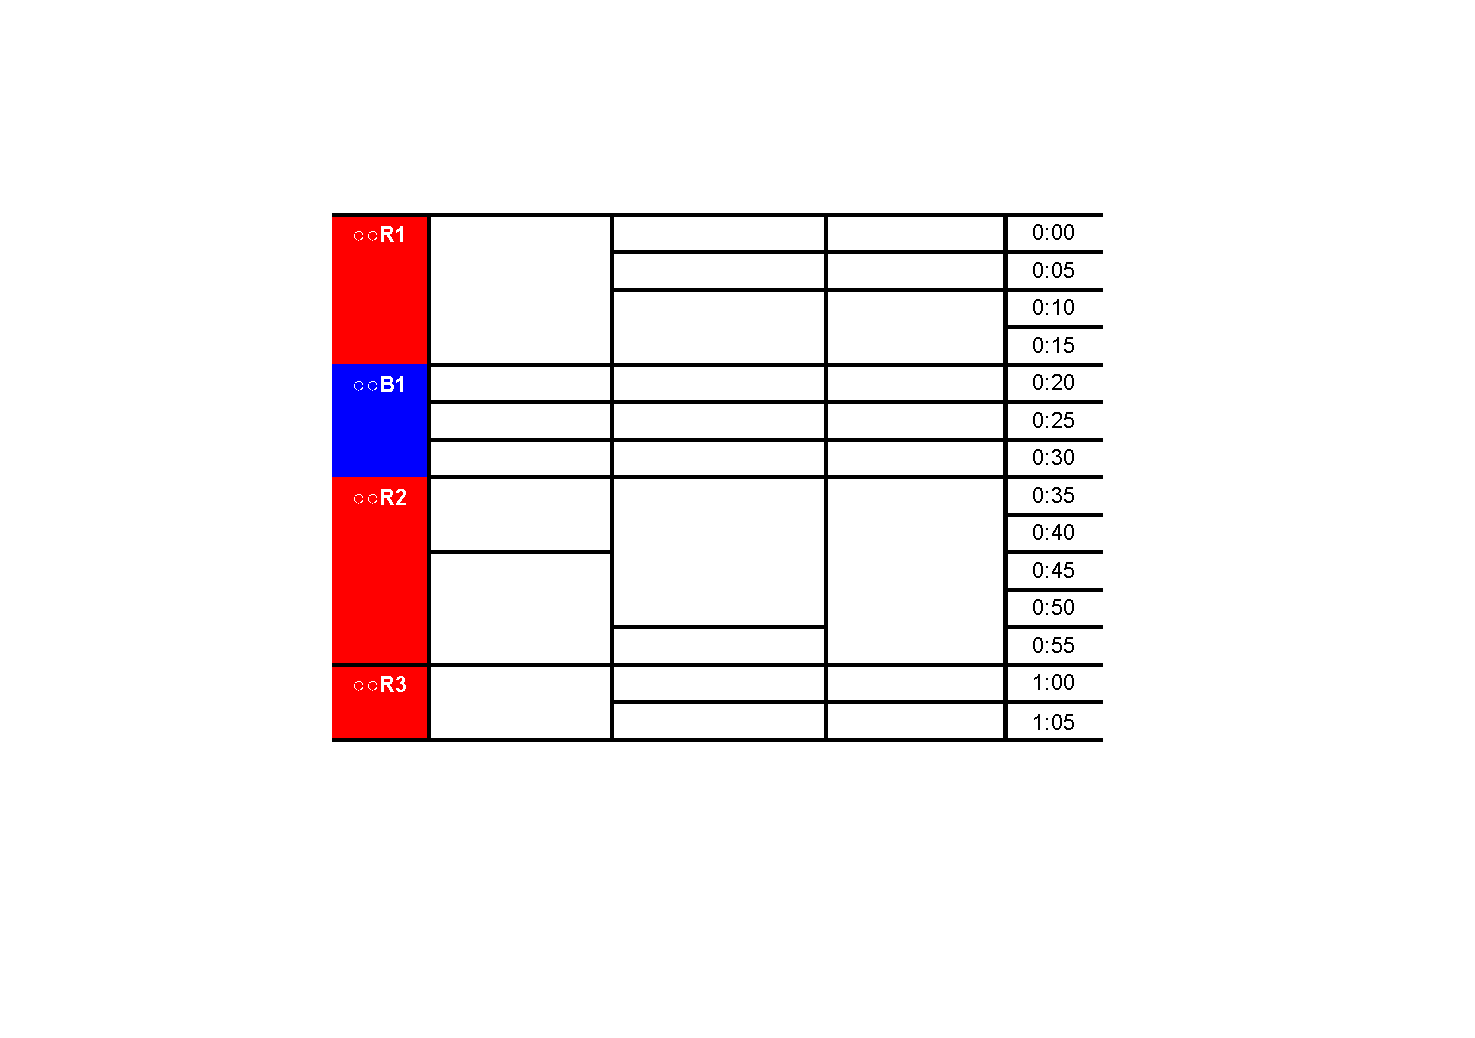
\includegraphics[width=\hsize]{fig/fig1-RB.pdf}
	\caption{被験者の命名シーンとラベルづけの例}
	\label{fig:rb}
\end{figure}

%分析の表記方法として（図1），縦軸は対象作品の時間，横軸は被験者それぞれの場面分けとなる．

% 分析する際，どの場面の部分のことを指しているのか理解できるように場面のラベル付けを行った．ラベル付けは，被験者全員の場面分けが同じ時間で区切られている場合は青で色付けしBを付与し，異なる場合は赤で色付けしRを付与する．

% 以降では，対象作品の概要と分析の結果し，場面分けの要因をまとめていく．
\subsection{The Two Mouseketeers}\label{sec:two_mouse}
\subsubsection{あらすじ}
この物語は，1952年に公開されたアカデミー賞受賞の短編アニメーション\red{である\cite{mouseketeers}}．
中世フランスを舞台に，ジェリーとニブルスは小さな剣を持った勇敢な「マウスケティア」として，トムが見張る宮廷の豪華な食事を盗もうとする．トムは晩餐を守る猫の役割を果たすが，ジェリーたちは次々と知恵を駆使してトムを出し抜き，騒動を巻き起こす\red{というものである}．

この物語に登場する灰色のネズミは表記ゆれによりタフィーとニブルスという二つの名前がある．本稿では，灰色のネズミはタフィーとする．


\subsubsection{結果}
\red{
	まず，
	7分40秒の映像に対し，
	全部で17のグループに分けることができた．このうち，B群は10グループ，R群は13グループである．
}

\red{
	B群については，区切り方は同じでも，名称の付け方が３人とも異なっている場面がある．例えば，TTB3（\figref{scene-mouseketeers}）は，タフィーとジェリーの屋外でのやりとりから，建物内にいるトムの場面に変わるところであるが，その名称については三者三様に「トム登場」「ジェリー指さす」「窓にトムと飼い主の情景が映る」としており，着目している視点が異なっていることがわかる．
	この他，B群の中で特徴的なものとして，以下のようなものがある．
}


\begin{itemize}
	\item TTB5：トムとジェリーとタフィーがその物語の中で初めて関わる重要な場面であるため共通して同じ場面分けになったのではないかと考える．
	\item TTB9：タフィーが仕掛けた大砲を発射することによってトムと二匹のネズミとの戦いに決着がつくので物語の中でも印象深い場面となり同じになるのではないかと考える．
\end{itemize}


\red{
	R群は，被験者によって区切り方が異なった場面である．
	下記に，特徴的なものを挙げる．
}
\begin{figure}[tb]
	\centering
	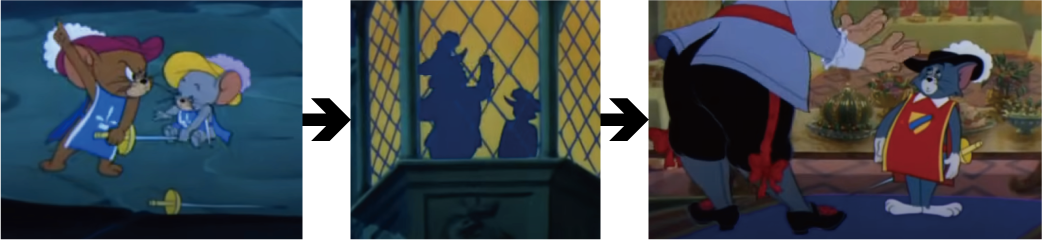
\includegraphics[width=\hsize]{fig/scene-mouseketeers.png}
	\caption{「The Two Mouseketeers」でのシーン遷移（TTB2）}
	（画像は文献\cite{mouseketeers}より引用）
	\label{scene-mouseketeers}
\end{figure}

\begin{itemize}
	\item TTR2：ジェリーとタフィーが静かにしないといけない状況ということを意識した場合細分化を行っているのではないか．
	\item TTR3：トムの飼い主からの指示の中身を重要視する場合細分化を行う．
	\item TTR5：ジェリーとタフィーが城に侵入するという場面は共通するが，細分化する場合は各登場人物が行っている行動を場面分けしただけだと考える．
	\item TTR7：コルクを当ててきた犯人を捜しにきたトムに対して，トムとタフィーが隠れるという場面であるが，隠れた後に場面転換して次の話になっている．そのため，隠れた後は何も起こっていない．その隠れるという動作に意識したかしていないかで細分化が変ってくる．
	\item TTR8：タフィー視点とタフィーからトム視点に変わっている2パターン存在し，視点が変わっている場面分けの方が細分化される．
	\item TTR10：細分化している方はトムとジェリーの戦いの内容まで意識していて，そうでないほうは戦いの流れを記載している．つまり二匹の戦い自体を広い視点か狭い視点かによって細分化が決まる．
	\item TTR11：細分化している方はトムの服に対しての記載がある．
\end{itemize}

\red{
	\figref{fig:two}（p. \pageref{fig:two}）に，「The Two Mouseketeers」の場面分け結果を示す．
}
\begin{figure*}[p]
	\centering
	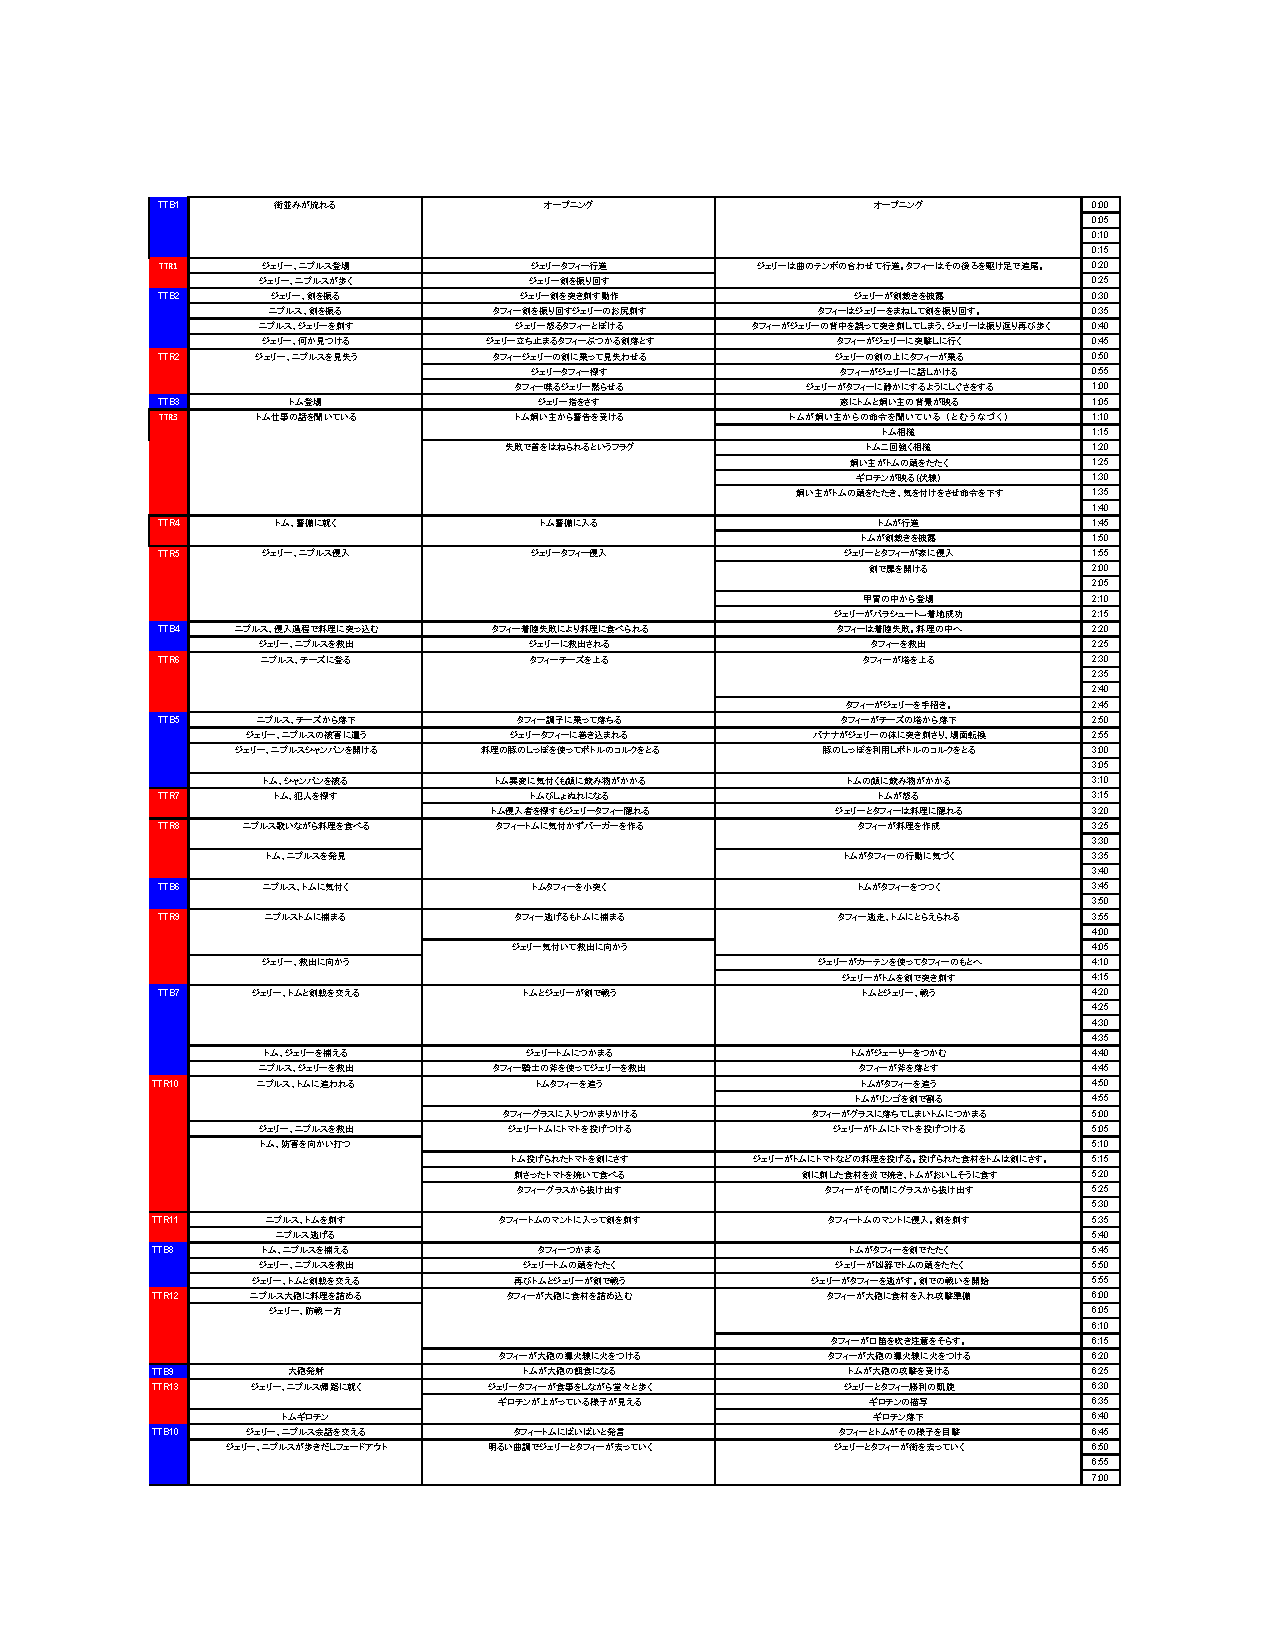
\includegraphics[width=.8\hsize]{fig/fig2-The_Two_Mouseketeers.pdf}
	\caption{The Two Mouseketeers分析結果}
	\label{fig:two}
\end{figure*}



\begin{figure*}[p]
	\centering
	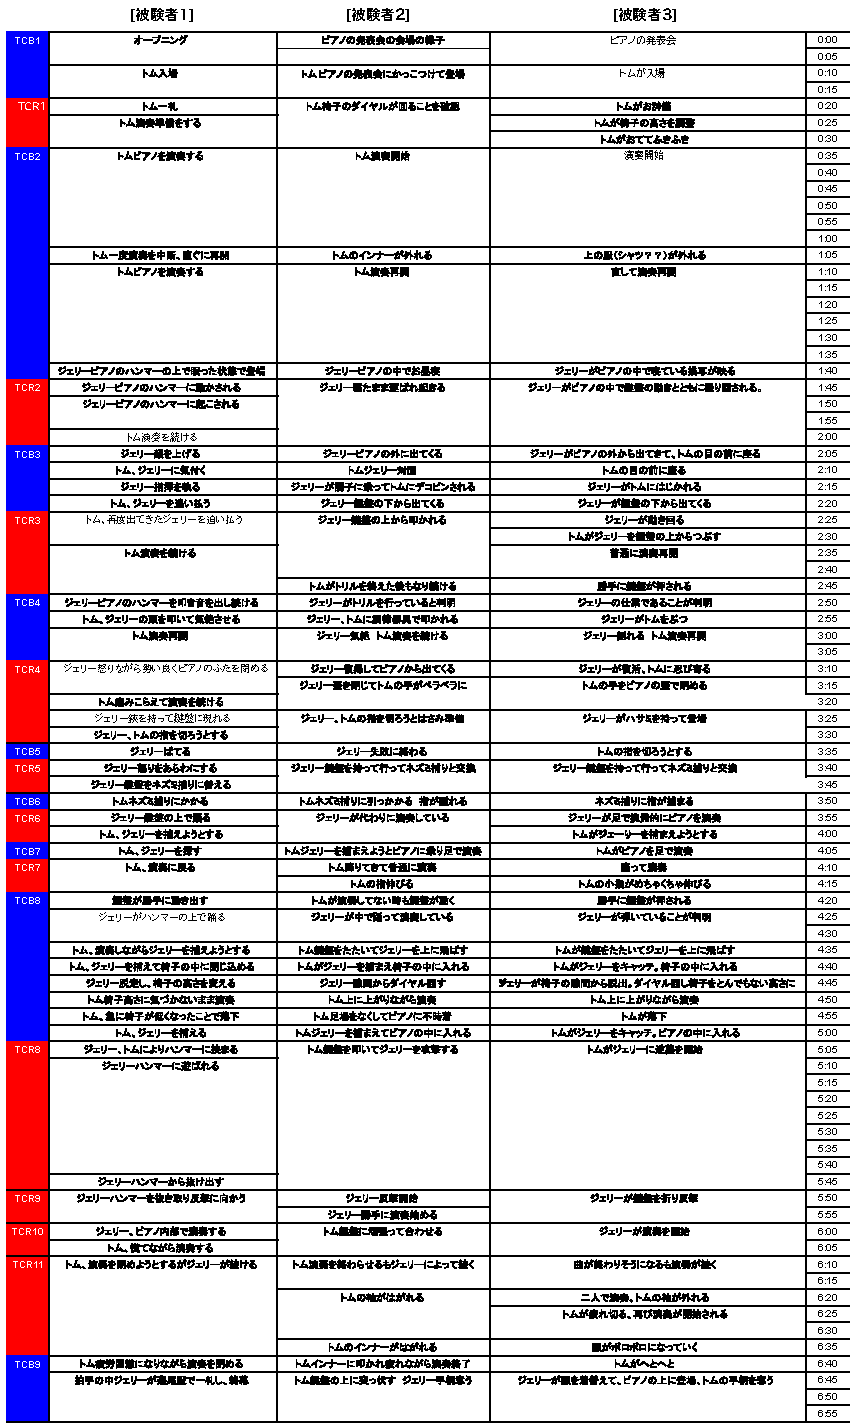
\includegraphics[width=.8\hsize]{fig/fig3-The_Cat_Concerto.pdf}
	\caption{The Cat Concerto分析結果}
	\label{fig:concerto}
\end{figure*}

\subsection{The Cat Concerto}\label{sec:cat_concerto}
\subsubsection{あらすじ}
この物語は，1947年に公開された\tomjerry の短編アニメーションであり，アカデミー賞短編アニメ賞を受賞した作品である．内容として，トムが優雅なコンサートホールでピアニストとして舞台に立つ場面から始まる．彼は観客の前で「ハンガリー狂詩曲第2番」を演奏する．しかし，ピアノの内部にジェリーが住み着いており，演奏中に邪魔を始める．


\subsubsection{結果}
\figref{fig:concerto}に，「The Cat Concerto」の場面分け結果を示す．

\red{B群についての特徴を以下に挙げる．}

\begin{itemize}
	\item TCB2：トムの服に対しての記述に着目したい．これはのちにTCR11へ繋がる伏線と考えられる．
	\item TCB4：直前までの話の流れから，ジェリーがハンマーをたたいてピアノを鳴らしていることが判明する場面で\red{あり，物語前半の答え合わせとなる場面である．いずれの被験者も}共通して印象深く感じ\red{られ}たのではないかと思われる．
	\item TCB6：前の場面での結果\red{を示す部分となる．}被験者が一致して意識して観た場面だと考え\red{られ}る．
	\item TCB8：\red{約40秒間のという長さで}同じ分け方にな\red{った．}場面の名称は多少異なるが\red{，}主語と行動がどの場面も同じになっている．
\end{itemize}


次にR群について述べる．
\begin{itemize}
	\item TCR2:\red{被験者1のみが，}トムの行動\red{について言及するために場面を3つに分割している}．
	      トムの演奏\red{シーンでは，}トム自身\red{がまだ}ジェリーに気づいていない状態\red{であることが示唆される}．トムの行動\red{について言及するということは，被験者1は}第三者視点で物語を観ているのではないかと考え\red{られ}る．
	\item TCR4:ピアノのふたを閉めた後トムが演奏を続けたということを物語の中で重要視したかどうかで場面分けが変化する．
	\item TCR5:前の場面でトムに仕掛けたことが失敗に終わった後のジェリーが怒るという結果を意識するかどうかで変わる．
	\item TCR7:トムの行動を演奏とひとくくりと解釈しているのか，演奏の中のパフォーマンスとして解釈しているのかで細分化が決まってくる．
	\item TCR8:トムがジェリーに向けて敵意を向けていると解釈した場合攻撃や逆襲などで一つの場面分けになっているが，細分化している方は，トムがジェリーに対して行ったハンマーにされたことを記載している．
	\item TCR10:\red{このシーンを}細分化\red{した被験者1}は，ジェリーからトムへと視点が移動している\red{ことが示唆される}．
	\item TCR11:トムの演奏に対しての「疲労感」を意識するかどうかで，細分化するかどうかが変化\red{したものと考えられる}．トムの「疲労感」が表面化を表す袖が剥がれたり服がボロボロになったりする場面が追加されるのではないかと考える．
\end{itemize}


\subsection{The Missing Mouse}\label{sec:missing_mouse}
\subsubsection{あらすじ}
この物語は，1953年に公開された\tomjerry の短編アニメーションである．内容としてトムがジェリーを追いかける中で，ジェリーが白い塗料を浴びて真っ白なネズミに変身する話．ラジオで「危険な放射性ネズミが逃げた」というニュースを聞いたトムは，ジェリーをそのネズミだと勘違いし，大混乱に陥る．

\begin{figure*}[p]
	\centering
	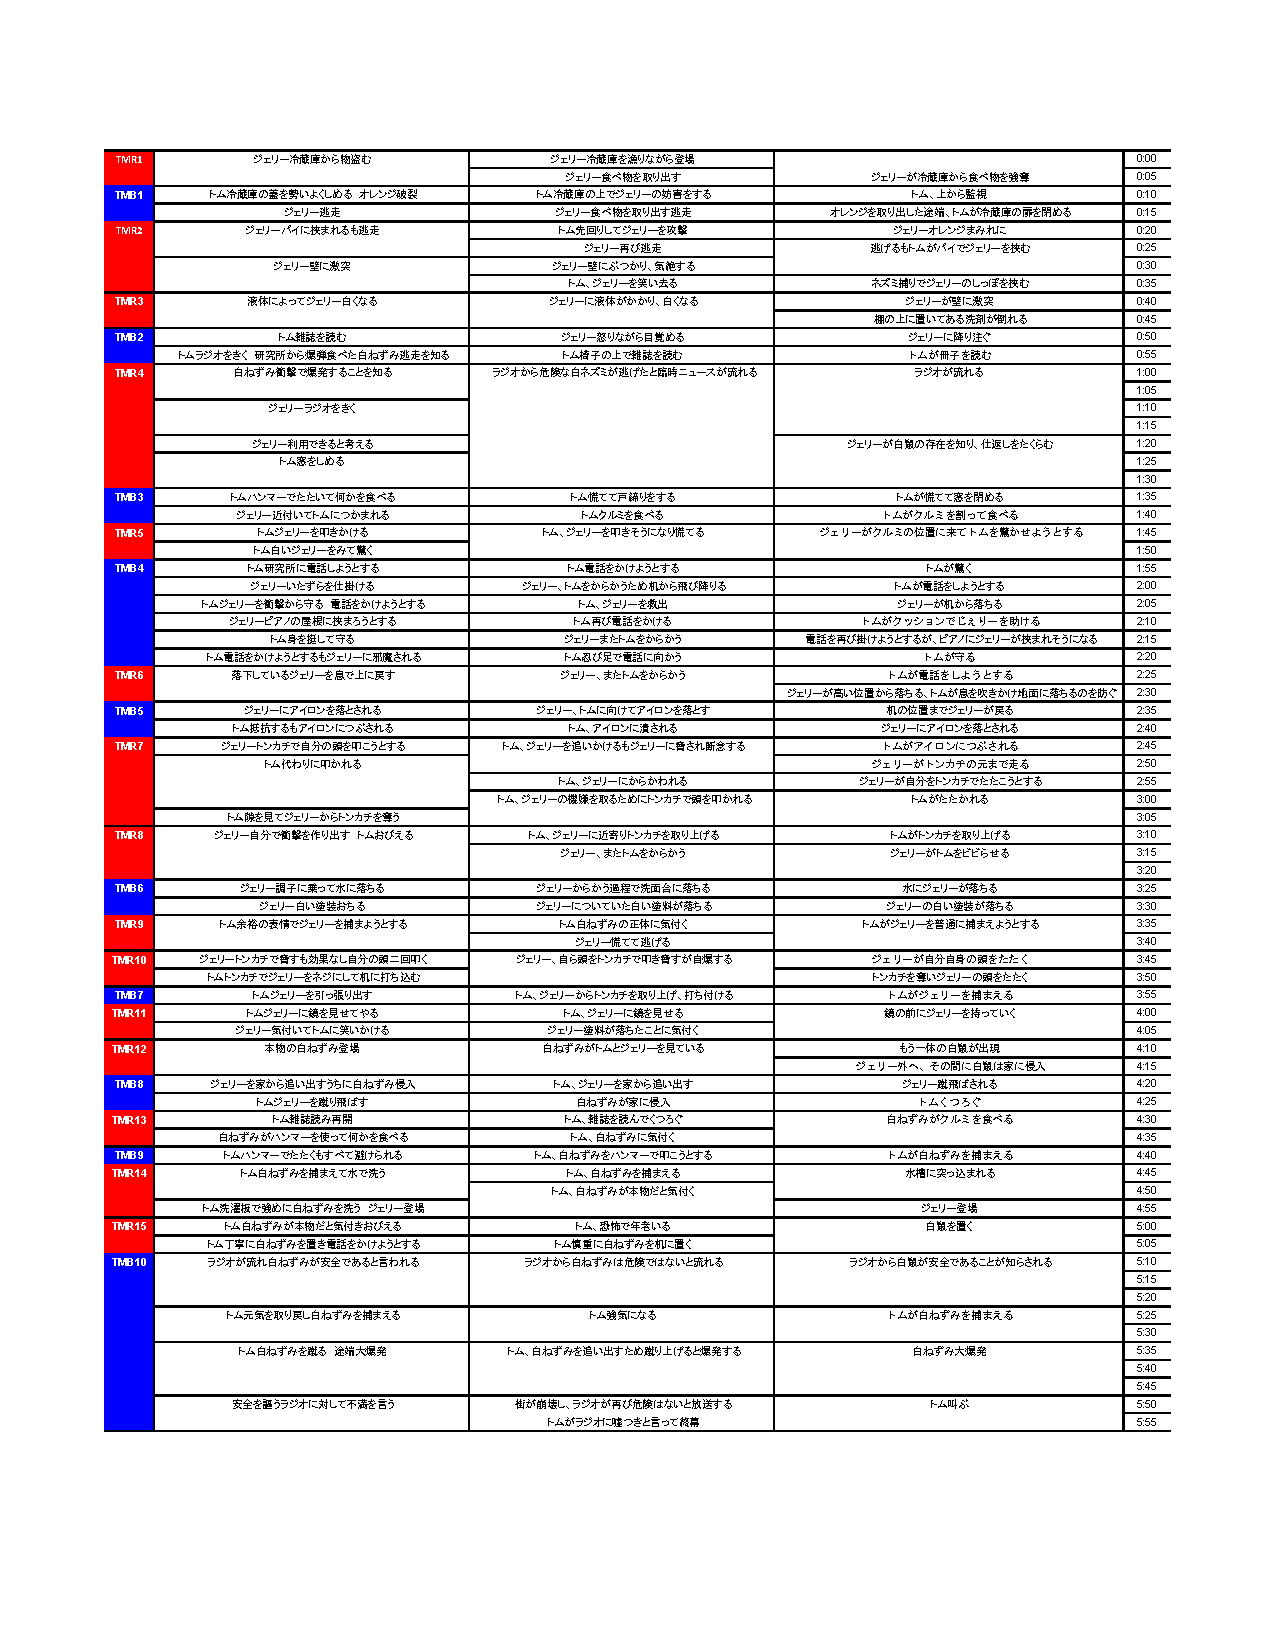
\includegraphics[width=\hsize]{fig/fig4-The_Missing_Mouse.pdf}
	\caption{The Missing Mouse分析結果}
	\label{fig:missing}
\end{figure*}
\subsubsection{結果}
\figref{fig:missing}に，「The Missing Mouse」の場面分け結果を示す．

B群についての特徴を以下に挙げる．

\begin{itemize}
	\item TMB4は，ジェリーを白ネズミと勘違いしているトムが爆発させないようにする場面は物語全体でも印象深いため共通するのではないかと考える．
	\item TMB6は，ジェリーの白い塗料が落ちトムがジェリーだと気づき，今までの立場が逆転する場面であるため同じになるのではないかと考える．
	\item TMB8は，白ネズミがジェリーだったと気づき家には白ネズミがいないと思っているトムに本物の白ネズミが登場する場面であり，白ネズミが話全体で重要であると解釈したためではないかと考える．
\end{itemize}
次に，次にR群について述べる．
\begin{itemize}
	\item TMR2:細分化していないほうは，ジェリーのみの視点であり，細分化している方は，トムからジェリーへ移動したり逆にジェリーからトムへと視点が移動していたりする．
	\item TMR3:ジェリーが白くなる部分は一緒だが，なぜ白くなったのかの経緯を意識すると細分化が行われる．
	\item TMR4:ジェリーが白いネズミの放送を聞いてその後にトムに対しての行動の理由となるものを意識する場合細分化が行われる．
	\item TMR9:トムがジェリーを捕まえようとした後のジェリーの行動を意識するかどうかで細分化されるか決まる．
	\item TMR11:「ジェリーが鏡を見る」＝「塗料が落ちることに気づく」とするかで塗料が落ちることに気づく場面を設定するか変っていく．
	\item TMR15:白ネズミが本物と気づいた後の老いていくトムの反応を重要視するかで細分化が変っていく．
\end{itemize}


\subsection{Mouse Trouble}\label{sec:mouse_trouble}
\subsubsection{あらすじ}
この物語は，1944年に公開された\tomjerry の短編アニメーションであり，アカデミー賞短編アニメ部門を受賞した作品である．内容としては，トムは，家にいるジェリーを捕まえるために「How to Catch a Mouse」（ネズミ捕獲の秘訣）という本を手に入れ，その指示を忠実に実行しようとする．しかし，ジェリーはトムの企みをことごとく見抜き，巧妙に切り抜けていく．

\begin{figure*}[p]
	\centering
	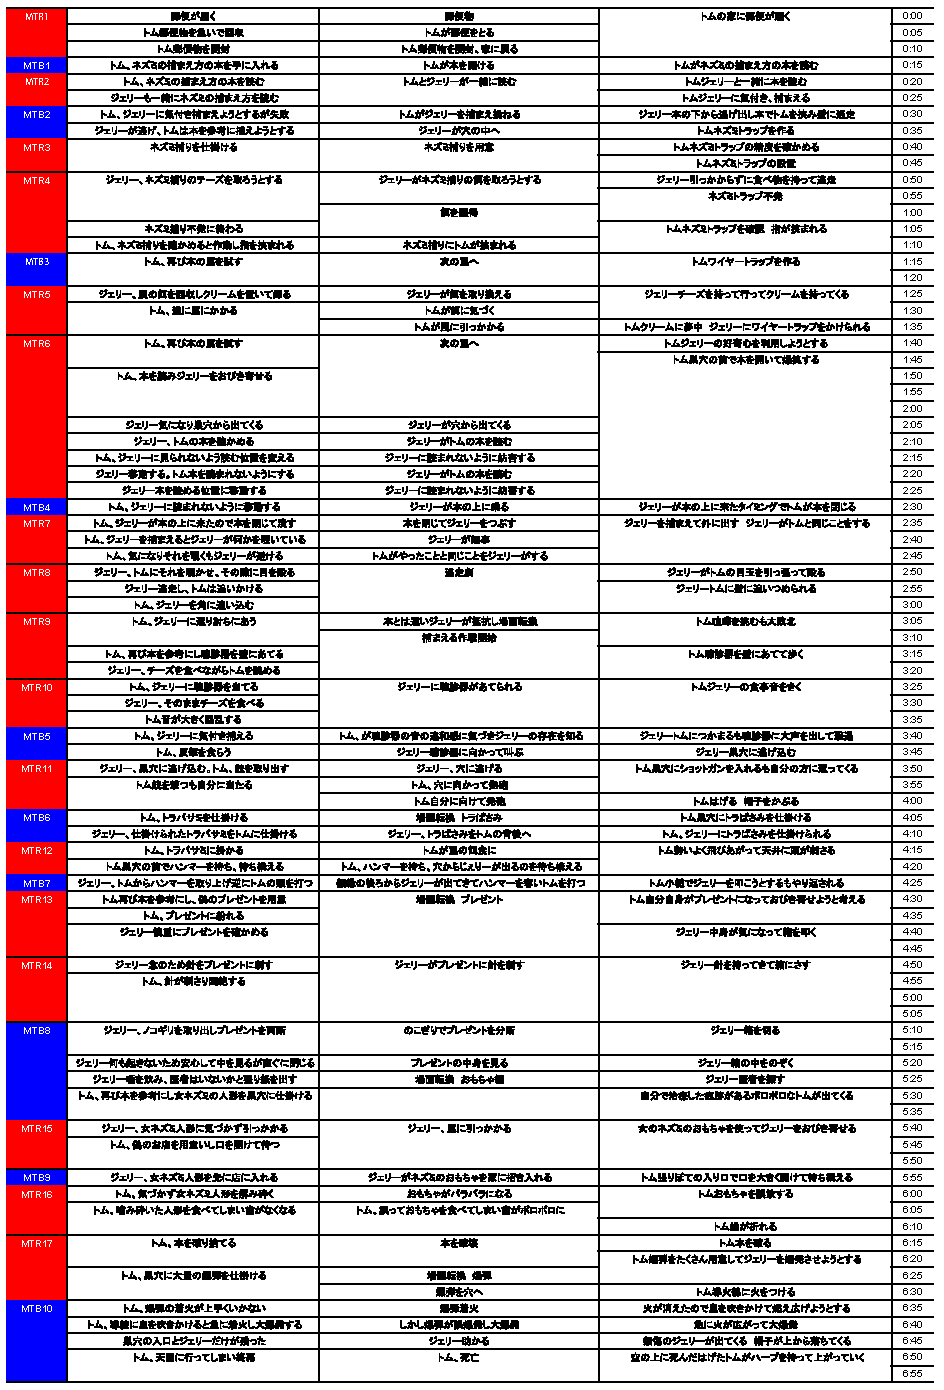
\includegraphics[width=.9\hsize]{fig/fig5-Mouse_Trouble.pdf}
	\caption{Mouse Trouble分析結果}
	\label{fig:trouble}
\end{figure*}

\subsubsection{結果}
\figref{fig:trouble}に，「Mouse Trouble」の場面分け結果を示す．

B群についての特徴を以下に挙げる．
\begin{itemize}
	\item MTB1は，物語の全体の流れとして本を参考にトムがジェリーを捕まえるために罠を仕掛ける．その始まりである本を初めて読む場面であり共通して重要な場面だと解釈したと考える．
	\item MTB3も，MTB1と同じように本を参考に罠を仕掛ける場面であるためMTB1と解釈が同じだと考える．
	\item MTB8は，トムが入っている箱をノコギリで分断するというショッキングな場面で，どの被験者にも強く印象に残ったためだと考える．
\end{itemize}

次に，R群について述べる．
\begin{itemize}
	\item MTR6は，細分化していないほうは，トムが行った行動のみで，細分化している方は，トムからジェリーへと視点が移動している．さらに細分化している方はジェリーが行った行動に対して細かく場面分けしている．
	\item MTR8は，トムとジェリーまとめての行動として場面を解釈しているか，各それぞれのキャラクターの行動としてみているかで細分化されるかが決まっていく．
	\item MTR9は，ジェリーを捕まえようとするトムの行動の行動に聴診器を使うという具体性がある場合細分化される．
	\item MTR10は，トムがジェリーに聴診器を当てた後のトムの反応を意識する場合細分化がされていく．
	\item MTR14は，ジェリーがトムの入っている箱に針を刺す場面であり，トムは映っていないがトムの悲鳴のような音が針を刺すたび鳴る．この音を意識した場合細分化が行われる．
	\item MTR15は，トムがどういった経緯でトム自身が仕掛けた罠に引っかかるのかを意識するかどうかで細分化が決まる．
\end{itemize}

\section{考察}

\subsection{対象作品を通じた全体の傾向}
\red{各}作品の同じ場面分けと異なる場面分けの個数を集計した\red{（\tabref{tab:kekka}）}．
すべての作品に言えることとして，同じ時間で場面分けしている\red{B群}よりも，異なる場面分け\red{をしているR群}のほうが多いという結果になった．


各対象作品で場面分けが異なる要因があったが，特に頻出した要素を対象作品ごとにまとめた．表を見ると二種類あり登場人物の行動の関連性と鑑賞者の物語に対する視点となる．登場人物の行動の関連性が頻出した理由としては，頻出した作品に共通して言えるのはトムとジェリーが物語全体を通して対立し争い合って，トムとジェリーの戦いの内容の解釈が被験者によって異なったためだと考える．鑑賞者の物語に対する視点が頻出した理由としては，物語全体で1つの場面内に複数人の登場人物が出ることが多く被験者によって注目する登場人物にばらつきが出たからではないかと考える．

\begin{table}[t]
	\centering
	\caption{３人の被験者による場面分けの結果}
	\label{tab:kekka}
	\begin{tabular}{l|cc}
		\hline
		\multirow{2}{*}{対象作品} & B群                    & R群                     \\
		                      & \scriptsize{（同じ場面分け）} & \scriptsize{（異なる場面分け）} \\
		\hline
		The Two Mouseketeers  & 10                    & 13                     \\
		The Cat Concerto      & 9                     & 11                     \\
		The Missing Mouse     & 10                    & 15                     \\
		Mouse Trouble         & 10                    & 17                     \\
		\hline
	\end{tabular}\\
	\raggedleft {（単位：シーン数）}
\end{table}

% \begin{figure}[tb]
% 	\centering
% 	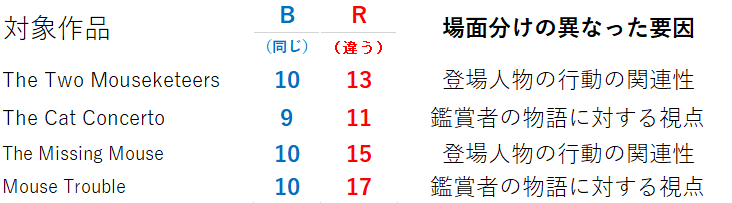
\includegraphics[width=\hsize]{fig/fig6-kekka.png}
% 	\caption{分析結果表}
% 	\label{fig:kekka}
% \end{figure}

\subsection{場面分けにおける要因}
被験者が観ている視点や行動が単一の場合，場面の細分化はあまり行われないことが多い．一方で，視点や行動が二つ以上存在する場合には，場面が細分化される傾向が顕著であった．特に，視点や行動を示す人物が変更される場合において，場面が細分化される可能性が高まることが確認された．以上の結果は，視点や行動の多様性が場面分けにおける細分化の程度に影響を与えることを示唆している．また，戦闘や演奏といった特定の行動を伴う場面における分析では，その行動が具体的である場合に場面が細分化されやすい傾向が確認された．たとえば，戦闘においては「剣を振る」という動作，演奏においては「鍵盤を叩く」という動作が具体的に描写される際に，場面が細分化される頻度が増加することが観察された．このことから，行動の具体性が場面分けにおける細分化に影響を与える要因の一つであると考えられる． The Cat Concertoのジェリーが怒る場面のような登場人物の感情が現れるところは被験者によって大きく場面分けが変わるポイントであった．

細分化されていない場面分けでは，The Two Mouseketeersのタフィーが放った大砲のようなその物語の状態が劇的に変わるような場面が共通して同じ場面分けになるのではないかと考えた．また，The Missing Mouseのジェリーの塗料が落ちて白ネズミではないことがトムにばれてるような今での登場人物間の関係が変わるような場面は共通して同じ場面になっていった．The Missing Mouseの最後の爆発やMouse Troubleの箱に入っているトムをジェリーがノコギリで分断する場面など強く印象に残るようなところは同じ場面分けになっている．細分化されていない場面に関する分析では，被験者全員が共通して同一の視点や行動を共有している傾向が見られた．このことは，視点や行動の一貫性が場面の細分化を抑制する要因として機能している可能性を示唆している．また，この傾向は，視点や行動が多様化した場合に場面が細分化されやすくなる結果とも整合的であると考えられる．



\subsection{場面転換における分割指針}
調査を通して，物語内の場面転換が行われた際場面分けをされていたとき，場面転換でも様々な要因で場面分けがされていることが分かった．以下でその要因を挙げていく．

\paragraph*{（1）時間的変化}
映像内での時間の経過は，場面の切り替えを示す重要な指標となる．時間の進行に応じて，物語の展開が新たな局面へと移行する場合，その変化点を基準に場面が区分されることが多い．たとえば，昼から夜へ，過去から現在へといった時間の変化が顕著に示される場合，場面が転換されたと判断できる．

\paragraph*{（2）空間的変化}
物語内での場面が展観される際には，空間の移動がしばしば伴う．登場人物が異なる場所へ移動することで，物語の新たな展開が生じ，場面が切り替わることが多い．例えば，屋内から屋外，都市から田舎といった舞台の変化は，視覚的にも場面の区分を明示する．

\paragraph*{（3）登場人物の変化}
映像内で登場する人物が変化することも，場面の切り替えを示す要素となる．特定の登場人物が画面上から姿を消し，新たな人物が現れることで，物語の視点や焦点が変わるため，場面の転換が認識される

\subsection{鑑賞者の視点}
各対象作品それぞれで考察した結果，場面分けが被験者それぞれで異なる場面分けが異なる要因が存在した．以下でその要因を挙げていく．

\paragraph*{（1）鑑賞者の物語に対する視点}
作品を鑑賞する際，鑑賞者が意識するか否かに関わらず，注目する登場人物は場面ごとに変化する．この注目の変化は，鑑賞者の視点や感情移入の対象が動的であることを示唆しており，作品の分析において重要な要素となる．分析を行う際には，鑑賞者が現在どの登場人物に注目しているのか，または特定の登場人物に注目していない場合には作品全体を俯瞰する第三者的視点で観ているのかを意識することが求められる．

\paragraph*{（2）行動の細分化}
「戦い」や「演奏」といった行動の大きなまとまりを捉えるか，あるいはそれを細分化した「剣をふるう」や「サビを弾く」といった個別の行動に焦点を当てるかは，分析の手法や目的に応じて変化する． 大きなまとまりとして行動を捉える場合，その行動全体の意図や結果に着目することが可能となる．一方で，細分化された行動を取り上げることで，具体的な動作や瞬間的な変化を明確にし，より詳細な洞察が得られる．これらのどちらの視点を選択するかは，分析の目的や求められる．

\paragraph*{（3）登場人物の感情}
作品において，登場人物たちが行動に移す背景にはさまざまな要因が存在する．その中でも，感情は行動を引き起こす重要な要因の一つであると考えられる．登場人物が抱いた感情がその行動の直接的な動機となっているのか，あるいは他の要因によるものなのかを見極めるこが大切である．感情に基づく行動は，登場人物の内面的な変化や心理的な背景を理解する上で鍵となり得る．一方で，感情に基づかない行動は，別の要因が関与している可能性を示唆する．したがって，分析者は各行動の背後にある要因を精査し，感情との関連性を考える必要がある．

\paragraph*{（4）登場人物の行動}
物語において，展開される行動は物語の進行を構築する重要な要素である．その中でも，特に劇的に場面が変化するような行動は，物語の構成において重要な役割を果たしている．そのような行動は，場面分けをする際，意識を向むけることが大切である．

\paragraph*{（5）登場人物の関係性}
物語において，登場人物間の関係が変化する場面は，物語の流れそのものに変化をもたらす重要な転換点である．このような関係性の変化，物語全体の展開において重要度が高いと考えられる．

場面分けを行う際には，登場人物間の関係がどのように変化し，それが物語の進行や構造にどのような影響を与えているかを意識することが重要である．

\paragraph*{（6）鑑賞者の感情}
作品を鑑賞する際，鑑賞者は喜びや感動といった多様な感情を抱く．その中でも，感情が大きく揺さぶられる場面は，鑑賞者に深い印象を与え，作品の記憶や評価に大きな影響を及ぼす．これらの場面は，物語のクライマックスや転換点であることが多く，鑑賞者の心に強く刻まれる．場面分けを行う際には，このような感情的揺さぶりが生じる場面を特に重視することが求められる．感情の高揚や変化が顕著である場面は，物語の流れやテーマを理解するうえで重要な役割を果たす．




\section{おわりに}
本研究では，場面分けに対して調査，比較分析，考察，提案を行ってきた．

調査として作品分析を行っている論文を収集し，場面分けの現状を調べた．

そのことを踏まえて短編アニメーション作品の\tomjerry を対象として被験者に場面分けを行ってもらい比較，考察を行った．
その考察を踏まえて場面分けに対しての要素として，場面転換，鑑賞者の物型に対する視点，行動の細分化，登場人物の感情や行動や関係性，鑑賞者の感情ではないかと考えた．
